\subsection{Slučaj upotrebe: Praćenje izlaznosti}

\subsubsection*{Kratak opis}
Član izborne komisije tokom trajanja glasanja prati broj studenata sa pravom glasa, broj studenata koji su glasali i procenat izlaznosti.

\subsubsection*{Akteri}
\begin{itemize}
    \item \textbf{Član izborne komisije} -- prati izlaznost tokom glasanja.
\end{itemize}

\subsubsection*{Preduslovi}
\begin{itemize}
    \item Član izborne komisije je prijavljen u sistem.
    \item Period glasanja za izabrane izbore je počeo.
\end{itemize}

\subsubsection*{Postuslovi}
\begin{itemize}
    \item Član komisije ima uvid u trenutnu izlaznost.
    \item Stanje sistema se ne menja.
\end{itemize}

\subsubsection*{Osnovni tok}
\begin{enumerate}
    \item Član komisije bira izbore i opciju \textbf{Praćenje izlaznosti}.
    \item Sistem proverava da je period glasanja počeo.
    \item Sistem računa broj studenata sa pravom glasa, broj studenata koji su glasali i procenat izlaznosti.
    \item Sistem prikazuje trenutnu izlaznost.
    \item Član komisije prati izlaznost i, po potrebi, osvežava prikaz. Tok se tada nastavlja od koraka 3.
\end{enumerate}

\subsubsection*{Alternativni tokovi}
\begin{enumerate}[label=\textbf{A\arabic*.}]
    \item \textbf{Glasanje još nije počelo.} Ako u koraku 2 period glasanja još nije počeo, sistem prikazuje poruku da glasanje još nije počelo. Slučaj upotrebe se završava.
\end{enumerate}

\subsubsection*{Dodatne informacije}
Sistem prikazuje samo zbirne podatke o izlaznosti. Tokom glasanja nije dostupan uvid u to za koju su listu studenti glasali niti koji su studenti glasali, čime se čuva tajnost glasanja.

\begin{figure}[H]
    \centering
    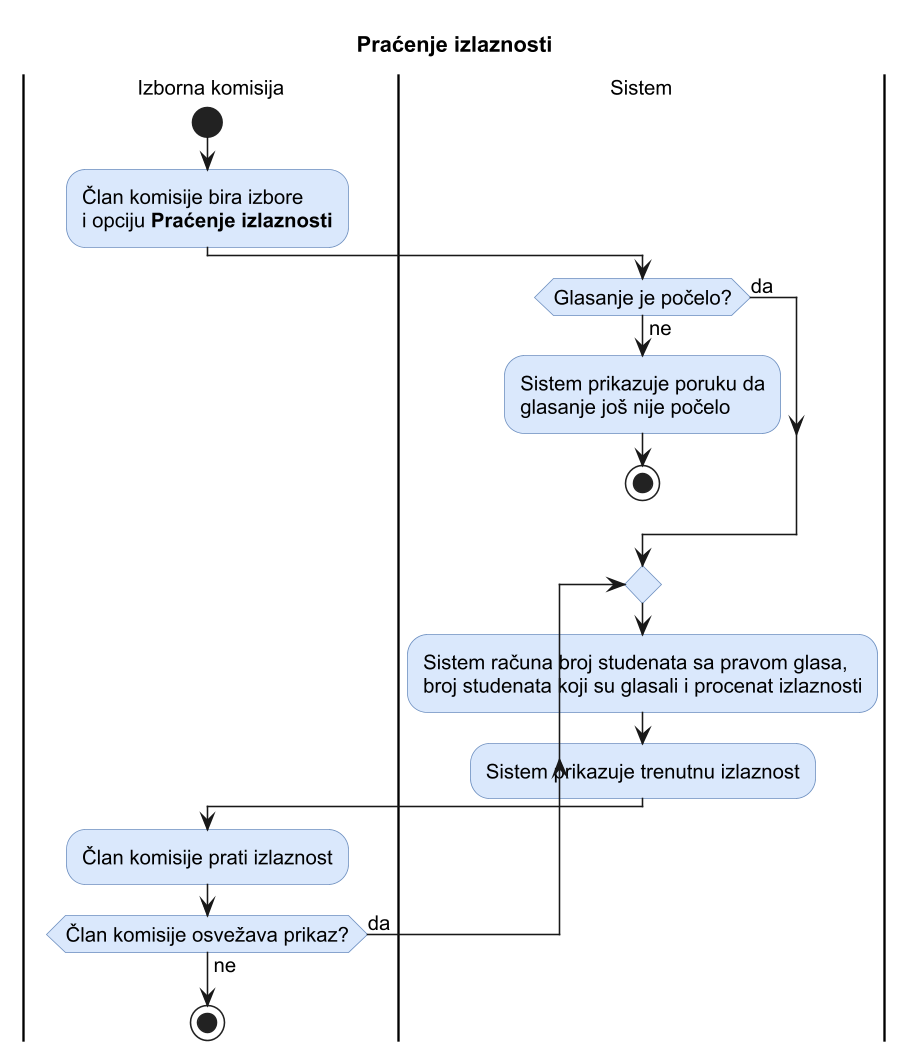
\includegraphics[width=0.7\textwidth]{aktivnosti_pracenje_izlaznosti.png}
    \caption{Dijagram aktivnosti: Praćenje izlaznosti}
    \label{fig:pracenje_izlaznosti}
\end{figure}

\newpage
